\newpage
\section{Finite element analysis}

\subsection{Finite element model}
Model construction

\subsubsection{Geometry}

CAD, 2D Axisymmetric

\subparagraph*{Spec and variability}
Check real data
\begin{figure}[h!]	
	\centering
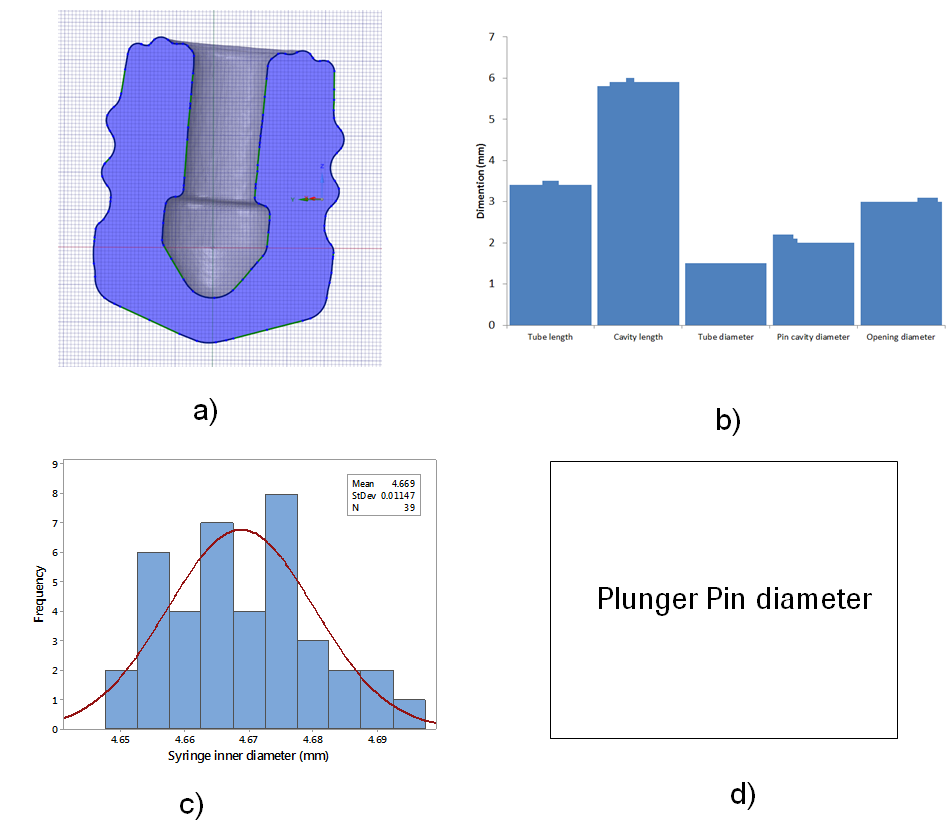
\includegraphics[height=11cm]{img/spec.PNG}
   \caption{Statistics of the measured factors . TO INTEGRATE: scanned stoppers, and their dimensions}
 \label{fgr:PFS}
\end{figure}

\newpage

\subsubsection{Meshing \& Loading}

There are two loading both controlled by displacement and they are first the barrel and then the plunger. The center of reference is the stopper and in order to avoid to simulate the whole stoppering step the stopper position is already there while the syringe is effectively larger thus not touching and not compressing the stopper. The other alternative is to start directly with the original barrel radius however this caused non convergence.

\begin{figure}[h!]	
	\centering
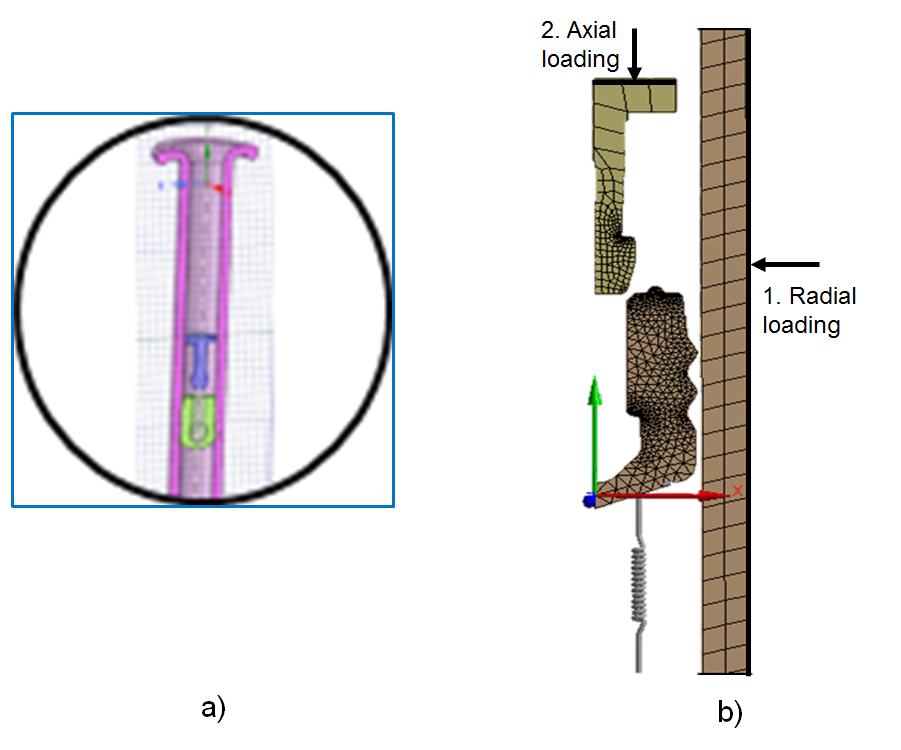
\includegraphics[height=7cm]{img/meshing.PNG}
   \caption{Stopper CAD and scan}
 \label{fgr:PFS}
\end{figure}


\subsubsection{Air bubble}
The air bubble is described by basic thermodynamic laws. FEM doesn't have these and thus there has to be an alternative to describe this and there are some possibilities. Basically, the air bubble pressure depends on its position.
Spring
Elastic material/ material young-s modulus
Challenge spring, nonlinear


\begin{figure}[h!]	
	\centering
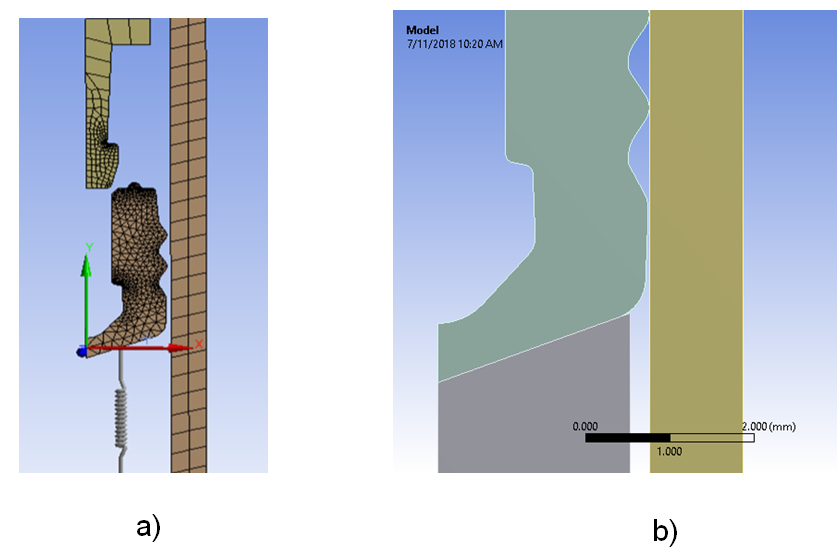
\includegraphics[height=7cm]{img/air.PNG}
   \caption{3D into 2D model}
 \label{fgr:PFS}
\end{figure}

\begin{equation}
\frac{F}{S}=Y\frac{\Delta L}{L}
\end{equation}

\newpage
\subsubsection{Material Data}
Sample, cutting, testing, ASTM, Data fitting

\begin{figure}[h!]	
	\centering
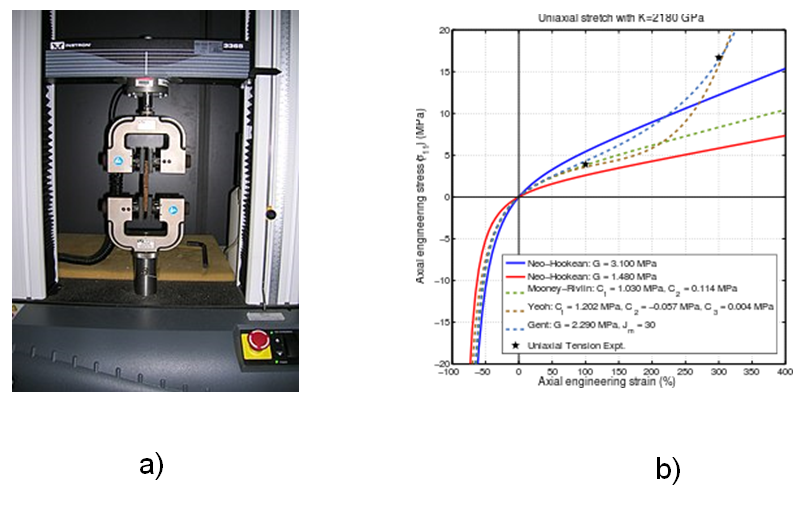
\includegraphics[height=7cm]{img/matdata.PNG}
   \caption{Data and model fitted}
 \label{fgr:PFS}
\end{figure}
Neo Hookean Model / Mooney Rivlin

\newpage
\subsection{Convergence}
Given the nature of the problem the main tools are contact and numerical
\subsubsection{Contact definition}
The tricky part is the friction coefficient ratio.

\subparagraph*{Barrel - Stopper}
This resulted in the less problematic given the right loading approach. The Lagrange is the right tool as it is a classical asymmetric rigid - flexible type of contact. Lagrange delivers thus on the zero penetration condition. Given the smooth compression of the stopper 

\subparagraph*{Stopper - Plunger}
This contact was the most problematic as it caused numerous element distrotions. Penalty method was the way to go in terms of helping the resolution of the problem by imposing less strict boundary conditions with the stiffness coeff. 


\subsubsection{Numerical methods}
Unsymmetric newton raphson explicit, implicit 

\subsubsection{Instability state}
Snap-fit

\subsubsection{Adaptive remeshing}

\newpage
\subsection{Calibration \& Validation}
Static simulation: main tools easier but has limitations: it is not dynamic.

\subsubsection{Stopper compression}
\begin{figure}[h!]	
	\centering
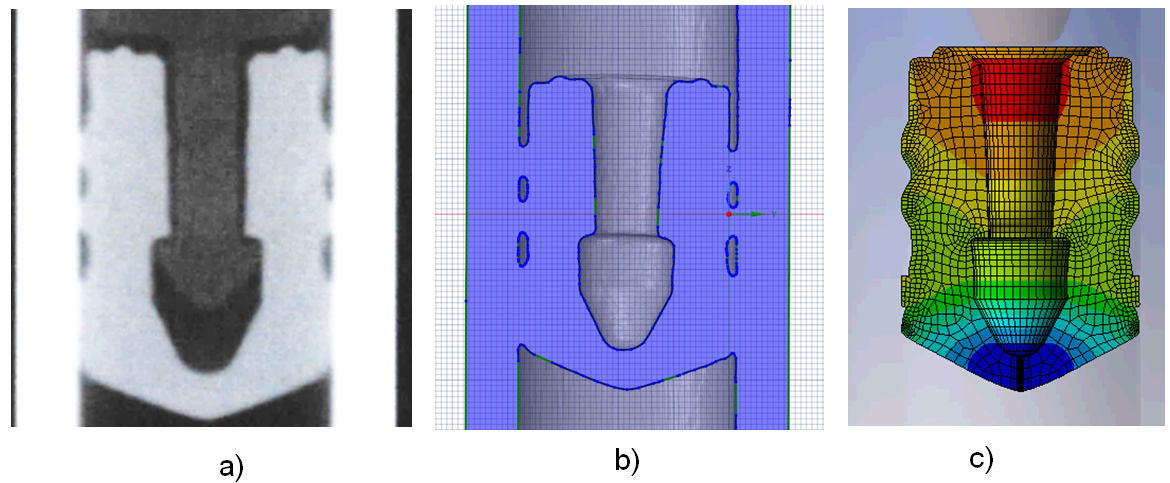
\includegraphics[height=7cm]{img/valicross.PNG}
   \caption{Stopper CT Scan and Simulation}
 \label{fgr:PFS}
\end{figure}

\newpage
\subsubsection{Plunger insertion}

\subparagraph{Frictionless}
Yadeyadeyada
\begin{figure}[h!]	
	\centering
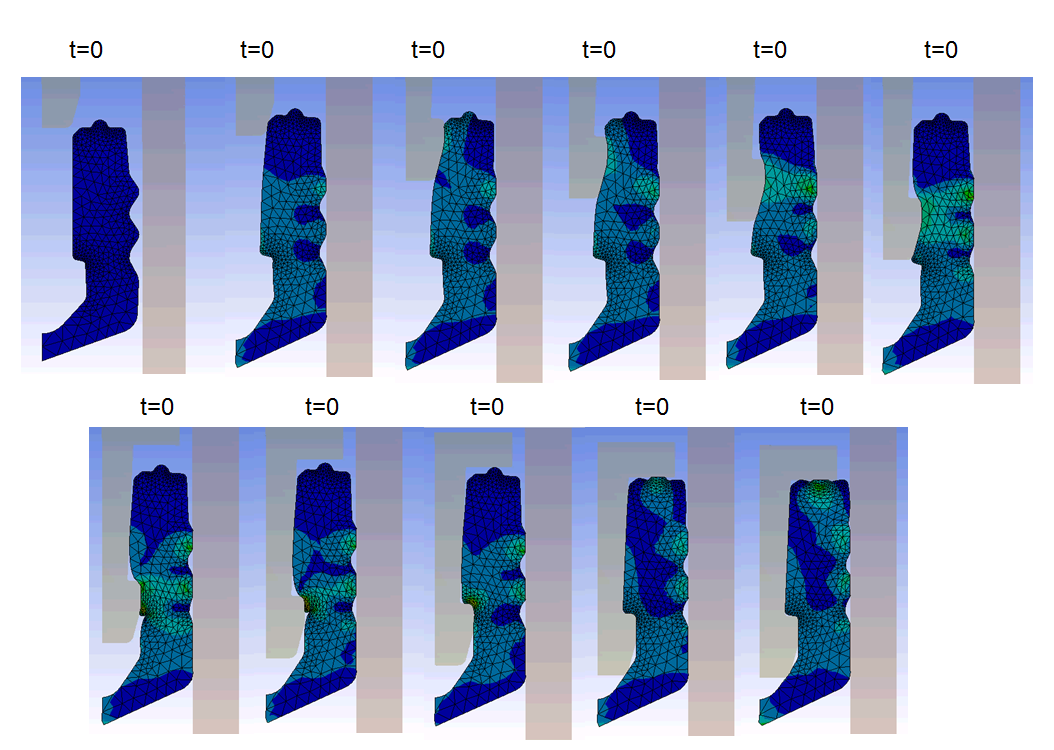
\includegraphics[height=11cm]{img/fricless.PNG}
   \caption{Frictionless plunger insertion sequence}
 \label{fgr:PFS}
\end{figure}

Insertion without problems but yields incorrect results.
\newpage
\subparagraph{Frictional}
Yadeyadeyada

\begin{figure}[h]	
	\centering
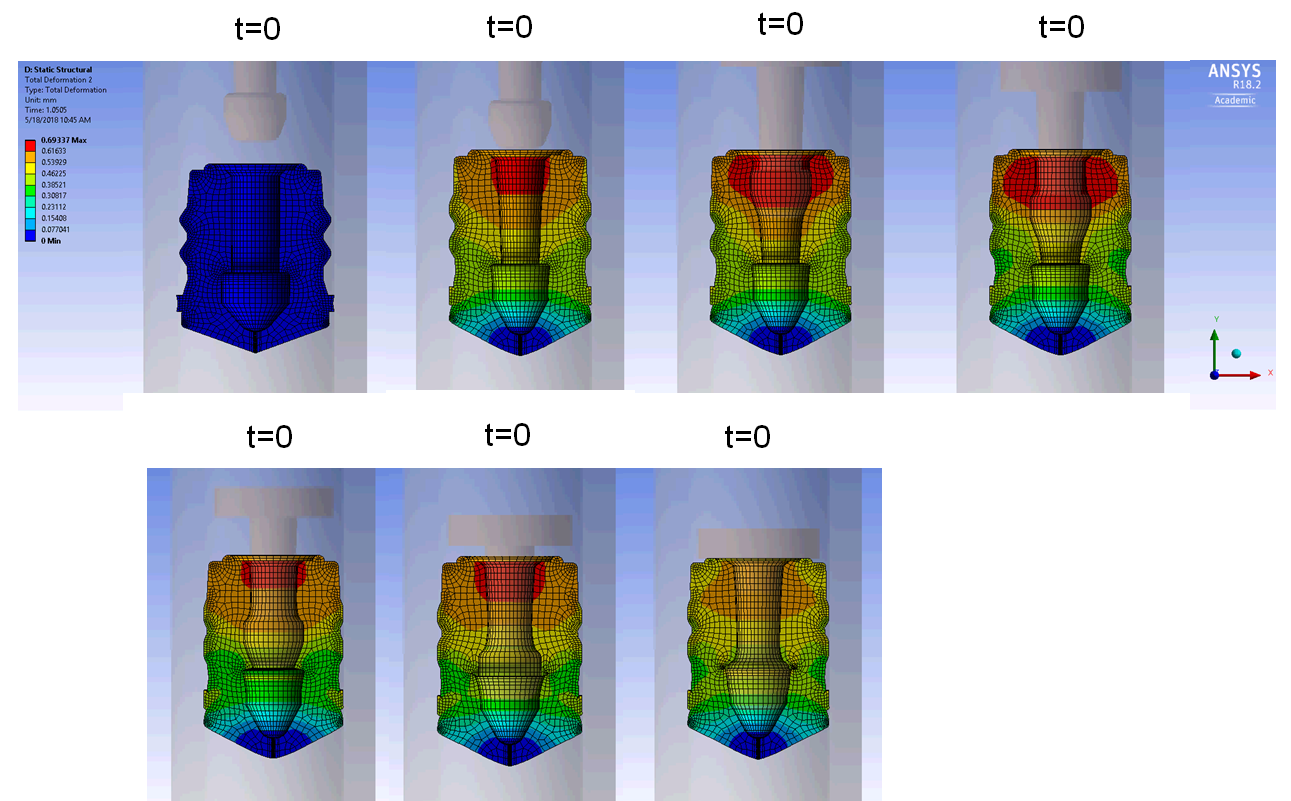
\includegraphics[height=10cm]{img/fric.PNG}
   \caption{Friction plunger insertion sequence}
 \label{fgr:PFS}
\end{figure}

 A singularity forms at the snap-in
 
\newpage
\subsubsection{Stopper movement}
Yadeyadeyada

\begin{figure}[h!]	
	\centering
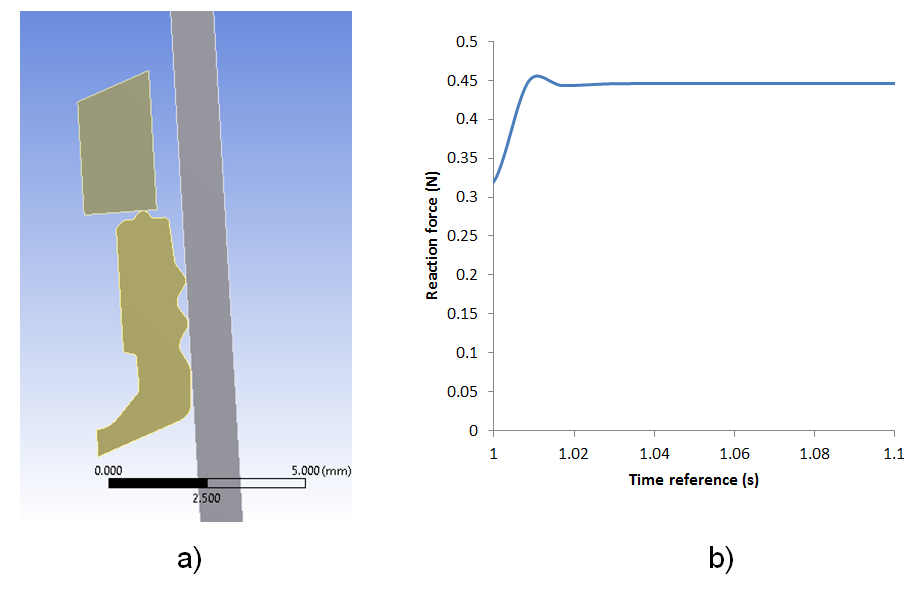
\includegraphics[height=9cm]{img/dyna.png}
   \caption{Simulation of stopper movement for break loose force and dynamic friction.}
 \label{fgr:PFS}
\end{figure}


\subsubsection{Model prediction accuracy}
Slow is OK, fast not OK


\newpage
\subsection{Sensitivity analysis}
Given the problematic snap-in, the focus was laid upon the maximum force and used as parameter for the sensitivity analysis. This is measured by the reaction force of the plunger displacement
\subsubsection{Geometry}
\subparagraph*{Barrel inner diameter}
\subparagraph*{Plunger pin diameter}
\subsubsection{Friction coefficients}

\begin{figure}[h!]	
	\centering
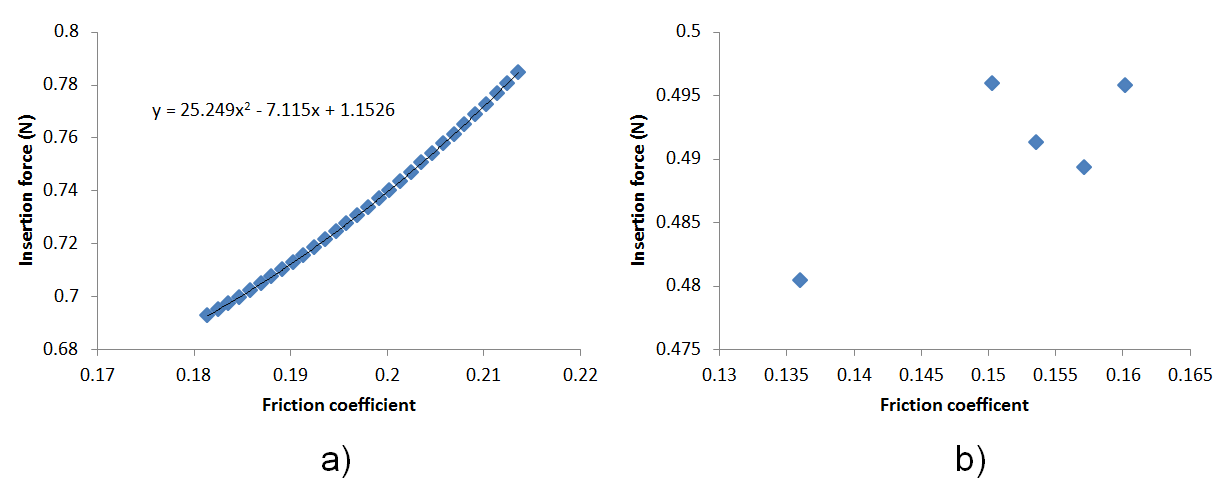
\includegraphics[height=6.5cm]{img/sens.PNG}
   \caption{Friction coeffs sensitivity analysis}
 \label{fgr:PFS}
\end{figure}


\newpage
\subsection{3D Model}
Challenges for meshing



